% https://www.overleaf.com/18225217jqvtscscccvs#/68889822/
% https://www.overleaf.com/18225348jztrfnwtzspz#/68890238/
% https://www.overleaf.com/read/hprgdrpcvvpm#/32910503/

%%%%%%%%%%%%%%%%%%%%%%%%%%%%%%%%%%%%%%%%% 
% Jacobs Portrait Poster
% LaTeX Template
% Version 1.0 (31/08/2015)
% (Based on Version 1.0 (29/03/13) of the landscape template
% 
% Created by:
% Computational Physics and Biophysics Group, Jacobs University
% https://teamwork.jacobs-university.de:8443/confluence/display/CoPandBiG/LaTeX+Poster
% 
% Further modified by:
% Nathaniel Johnston (nathaniel@njohnston.ca)
% 
% Portrait version by:
% John Hammersley
% 
% The landscape version of this template was downloaded from:
% http://www.LaTeXTemplates.com
% 
% License:
% CC BY-NC-SA 3.0 (http://creativecommons.org/licenses/by-nc-sa/3.0/)
% 
%%%%%%%%%%%%%%%%%%%%%%%%%%%%%%%%%%%%%%%%% 

\documentclass[final]{beamer}
\usepackage{graphicx}
\usepackage{enumitem}
\usepackage[framemethod=tikz]{mdframed}
% \usepackage[font=normalsize, justification=centering]{caption}
% \DeclareCaptionFont{normalsize}{\normalsize}
% \captionsetup{font=normalsize}


% Use the confposter theme supplied with this template
\usetheme{confposter}

% color styles
% Many more colors are available for use in beamerthemeconfposter.sty
% \setbeamercolor{block title}{fg=ngreen,bg=white}
% \setbeamercolor{block body}{fg=black,bg=white}
% \setbeamercolor{block alerted title}{fg=white,bg=dblue!70}
% \setbeamercolor{block alerted body}{fg=black,bg=dblue!10}

% \addtobeamertemplate{block begin}{\pgfsetfillopacity{0.0}}{\pgfsetfillopacity{1}}

% \usebackgroundtemplate{
% \begin{tikzpicture}
%   \path [outer color = green!10, inner color = blue!10]
%   (0,0) rectangle (\paperwidth,\paperheight);
% \end{tikzpicture}}

% Use the beamerposter package for laying out the poster (cm)
% https://github.com/deselaers/latex-beamerposter/blob/master/beamerposter.sty#L138
\usepackage[scale=1.6, size=custom, width=240, height=120]{beamerposter}

% Define the column widths and overall poster size

% To set effective sepwid, onecolwid and twocolwid values, first choose how many columns you want and how much separation you want between columns
% In this template, the separation width chosen is 0.024 of the paper width and a 4-column layout
% onecolwid should therefore be (1-(# of columns+1)*sepwid)/# of columns e.g. (1-(4+1)*0.024)/4 = 0.22
% Set twocolwid to be (2*onecolwid)+sepwid = 0.464
% Set threecolwid to be (3*onecolwid)+2*sepwid = 0.708
\newlength{\sepwid}
\newlength{\onecolwid}
\newlength{\twocolwid}
\newlength{\threecolwid}
\setlength{\paperwidth}{240cm}
\setlength{\paperheight}{120cm}
\setlength{\sepwid}{0.015\paperwidth} % Separation width (white space) between columns
\setlength{\onecolwid}{0.22\paperwidth} % Width of one column
\setlength{\twocolwid}{0.625\paperwidth} % Width of two columns
\setlength{\threecolwid}{0.90\paperwidth} % Width of three columns
\setlength{\topmargin}{-1in} % Reduce the top margin size

\addtobeamertemplate{block end}{}{\vspace*{2ex}} % White space under blocks
\addtobeamertemplate{block alerted end}{}{\vspace*{2ex}} % White space under highlighted (alert) blocks

\setlength{\belowcaptionskip}{2ex} % White space under figures
\setlength\belowdisplayshortskip{2ex} % White space under equations

\newcommand{\samelineand}{\qquad}

% http://mirror.hmc.edu/ctan/macros/latex/contrib/enumitem/enumitem.pdf
\setlist[itemize]{label=\textbullet,leftmargin=1.5cm}
\setlist[itemize,1]{itemsep=0.8cm}
\setlist[itemize,2]{itemsep=0.2cm}

\newcommand{\todo}[1]{\textbf{\textcolor{red}{TODO: #1}}}

\title{NautDB: Towards a Hybrid Runtime for Processing Compiled Queries}

% \author{\texorpdfstring{
% \begin{columns}
%   \column{0.33\linewidth}
%   \centering

%   \textbf{Samuel Grayson}\\[0.75ex]
%   Computer Science Department\\
%   University of Texas at Dallas\\
%       %   samuel.grayson@utdallas.edu

%   \column{0.33\linewidth}
%   \centering
%   \textbf{Kyle Hale}\\[0.5ex]
%   Computer Science Department\\
%   Illinois Institute of Technology\\
%       %   khale@cs.iit.edu

%   \column{0.3\linewidth}
%   \centering
%   \textbf{Boris Glavic}\\[0.75ex]
%   Computer Science Department\\
%   Illinois Institute of Technology\\
%       %   bglavic@cs.iit.edu
% \end{columns}
% }{}}
\author{\vspace{-4cm}Samuel Grayson\textsuperscript{1}, Kyle
  Hale\textsuperscript{2}, Boris Glavic\textsuperscript{2} \\}

% TODO: put emails on here
\institute{1 University of Texas at Dallas, 2 Illinois Insitute of Technology}

\graphicspath{{./imgs/}}

% LOGOS
\logo{%
    
\includegraphics[width=10cm,keepaspectratio]{dbgrouplogo.pdf}~%
    
\includegraphics[width=10cm,keepaspectratio]{hexsalablogo.pdf}%
}

\definecolor{mycolor}{rgb}{0.122, 0.435, 0.698}

\newmdenv[linewidth=10pt,innerlinewidth=0.5pt, roundcorner=40pt,linecolor=mycolor,innerleftmargin=26pt,
innerrightmargin=26pt,innertopmargin=26pt,innerbottommargin=26pt]{mybox}


% ----------------------------------------------------------------------------------------
\begin{document}

\begin{frame}[t] % The whole poster is enclosed in one beamer frame

  \begin{columns}[t]

    % spacer column
    \begin{column}{\sepwid}
    \end{column}

    % column 1
    \begin{column}{\onecolwid}
      \begin{block}{Abstract}
  \textbf{Goal:} to integrate specialization techniques from the OS
    community \buzzword{hybrid runtimes} and DB community
    \buzzword{compiled queries} for high-performance querying on
    \buzzword{big data}.

  \begin{itemize}

  \item Certain abstractions improve generality, but get in the way of
    performance at \buzzword{exascale computing}.

    
  \item In specific cases, give up flexibility and generality in exchange for performance.

    % Complex multi-layered abstractions behind generic interfaces in
    % the traditional OS and database software stack are getting in
    % the way of exploiting the characteristics of modern multi-core
    % systems to maximize performance.

  \item We prototype \buzzword{NautDB}: specialized using a
    \buzzword{hybrid runtime kernel} (based on the \buzzword{Nautilus
      Aerokernel}~\cite{HALE:2015:NAUTILUS}) and executing
    pre-compiled building-blocks.

    % for the parallel execution of \buzzword{compiled queries}, thus,
    % combining for the first time the concepts of hybrid runtimes and
    % compiled query processing developed by the operating system and
    % database communities.

  \item We demonstrate performance benefits in certain cases, while
    maintaining a simple interface for users.

  \end{itemize}
\end{block}

%%% Local Variables:
%%% mode: latex
%%% TeX-master: "main"
%%% End:

      \begin{block}{Motivation}




\underline{\textbf{Status quo}}
  \begin{itemize}
    \item Too many abstractions $\implies$ high-performance is difficult to achieve
    \item General purpose OS are not aware of the workload; app-programmer is.
    \item DBs already use specialized scheduling and memory management abstractions.
    \end{itemize}
 \alert{\textbf{Solution:} Give up flexibility and generality in exchange for performance.}\\[7mm]
    
\underline{\textbf{Specialized Hybrid Runtimes}}
    \begin{itemize}
    \item Kernel + Dataflow Runtime run in ring 0 (unikernel-like).
    \item Advances in multi-kernel environments allow physical \todo{(cite pisces)} resources to be split between a full-weight kernel and a hybrid runtime.
      % \item \alert{Unikernel-inspired design prevents the OS from `getting in the way' of the app-programmer.}
    \item {Unikernel-inspired design allows the app-programmer fine-grained control over the execution environment.}
      \begin{itemize}
      \item Control over scheduling $\implies$ no context-switches.
      \item Control over OS $\implies$ avoid interrupts $\implies$ faster and more predictable.
      \item No virtual memory $\implies$ huge page-sizes (1Gb) $\implies$ no TLB misses.
      \item Control over memory $\implies$ specialize memory-allocator for workload/application (see Fig.~ \ref{fig:1})
      \end{itemize}
    \end{itemize}

    \underline{\textbf{Compiled Query Processing}}
    \begin{itemize}
    \item Could be pre-compiled or JIT-compiled.
    \item {The app-programmer writes compiled code in the unikernel, giving them unfettered access HW.}
      \begin{itemize}
      \item Compose operators within a block $\implies$ avoid function-call overhead.
      \item Control HW $\implies$ NUMA-aware code.
      \end{itemize}
    \end{itemize}
\end{block}


%%% Local Variables:
%%% mode: latex
%%% TeX-master: "main"
%%% End:

    \end{column}

    % spacer column
    \begin{column}{\sepwid}
    \end{column}

    % column 2
    \begin{column}{\onecolwid}
      \begin{figure}
        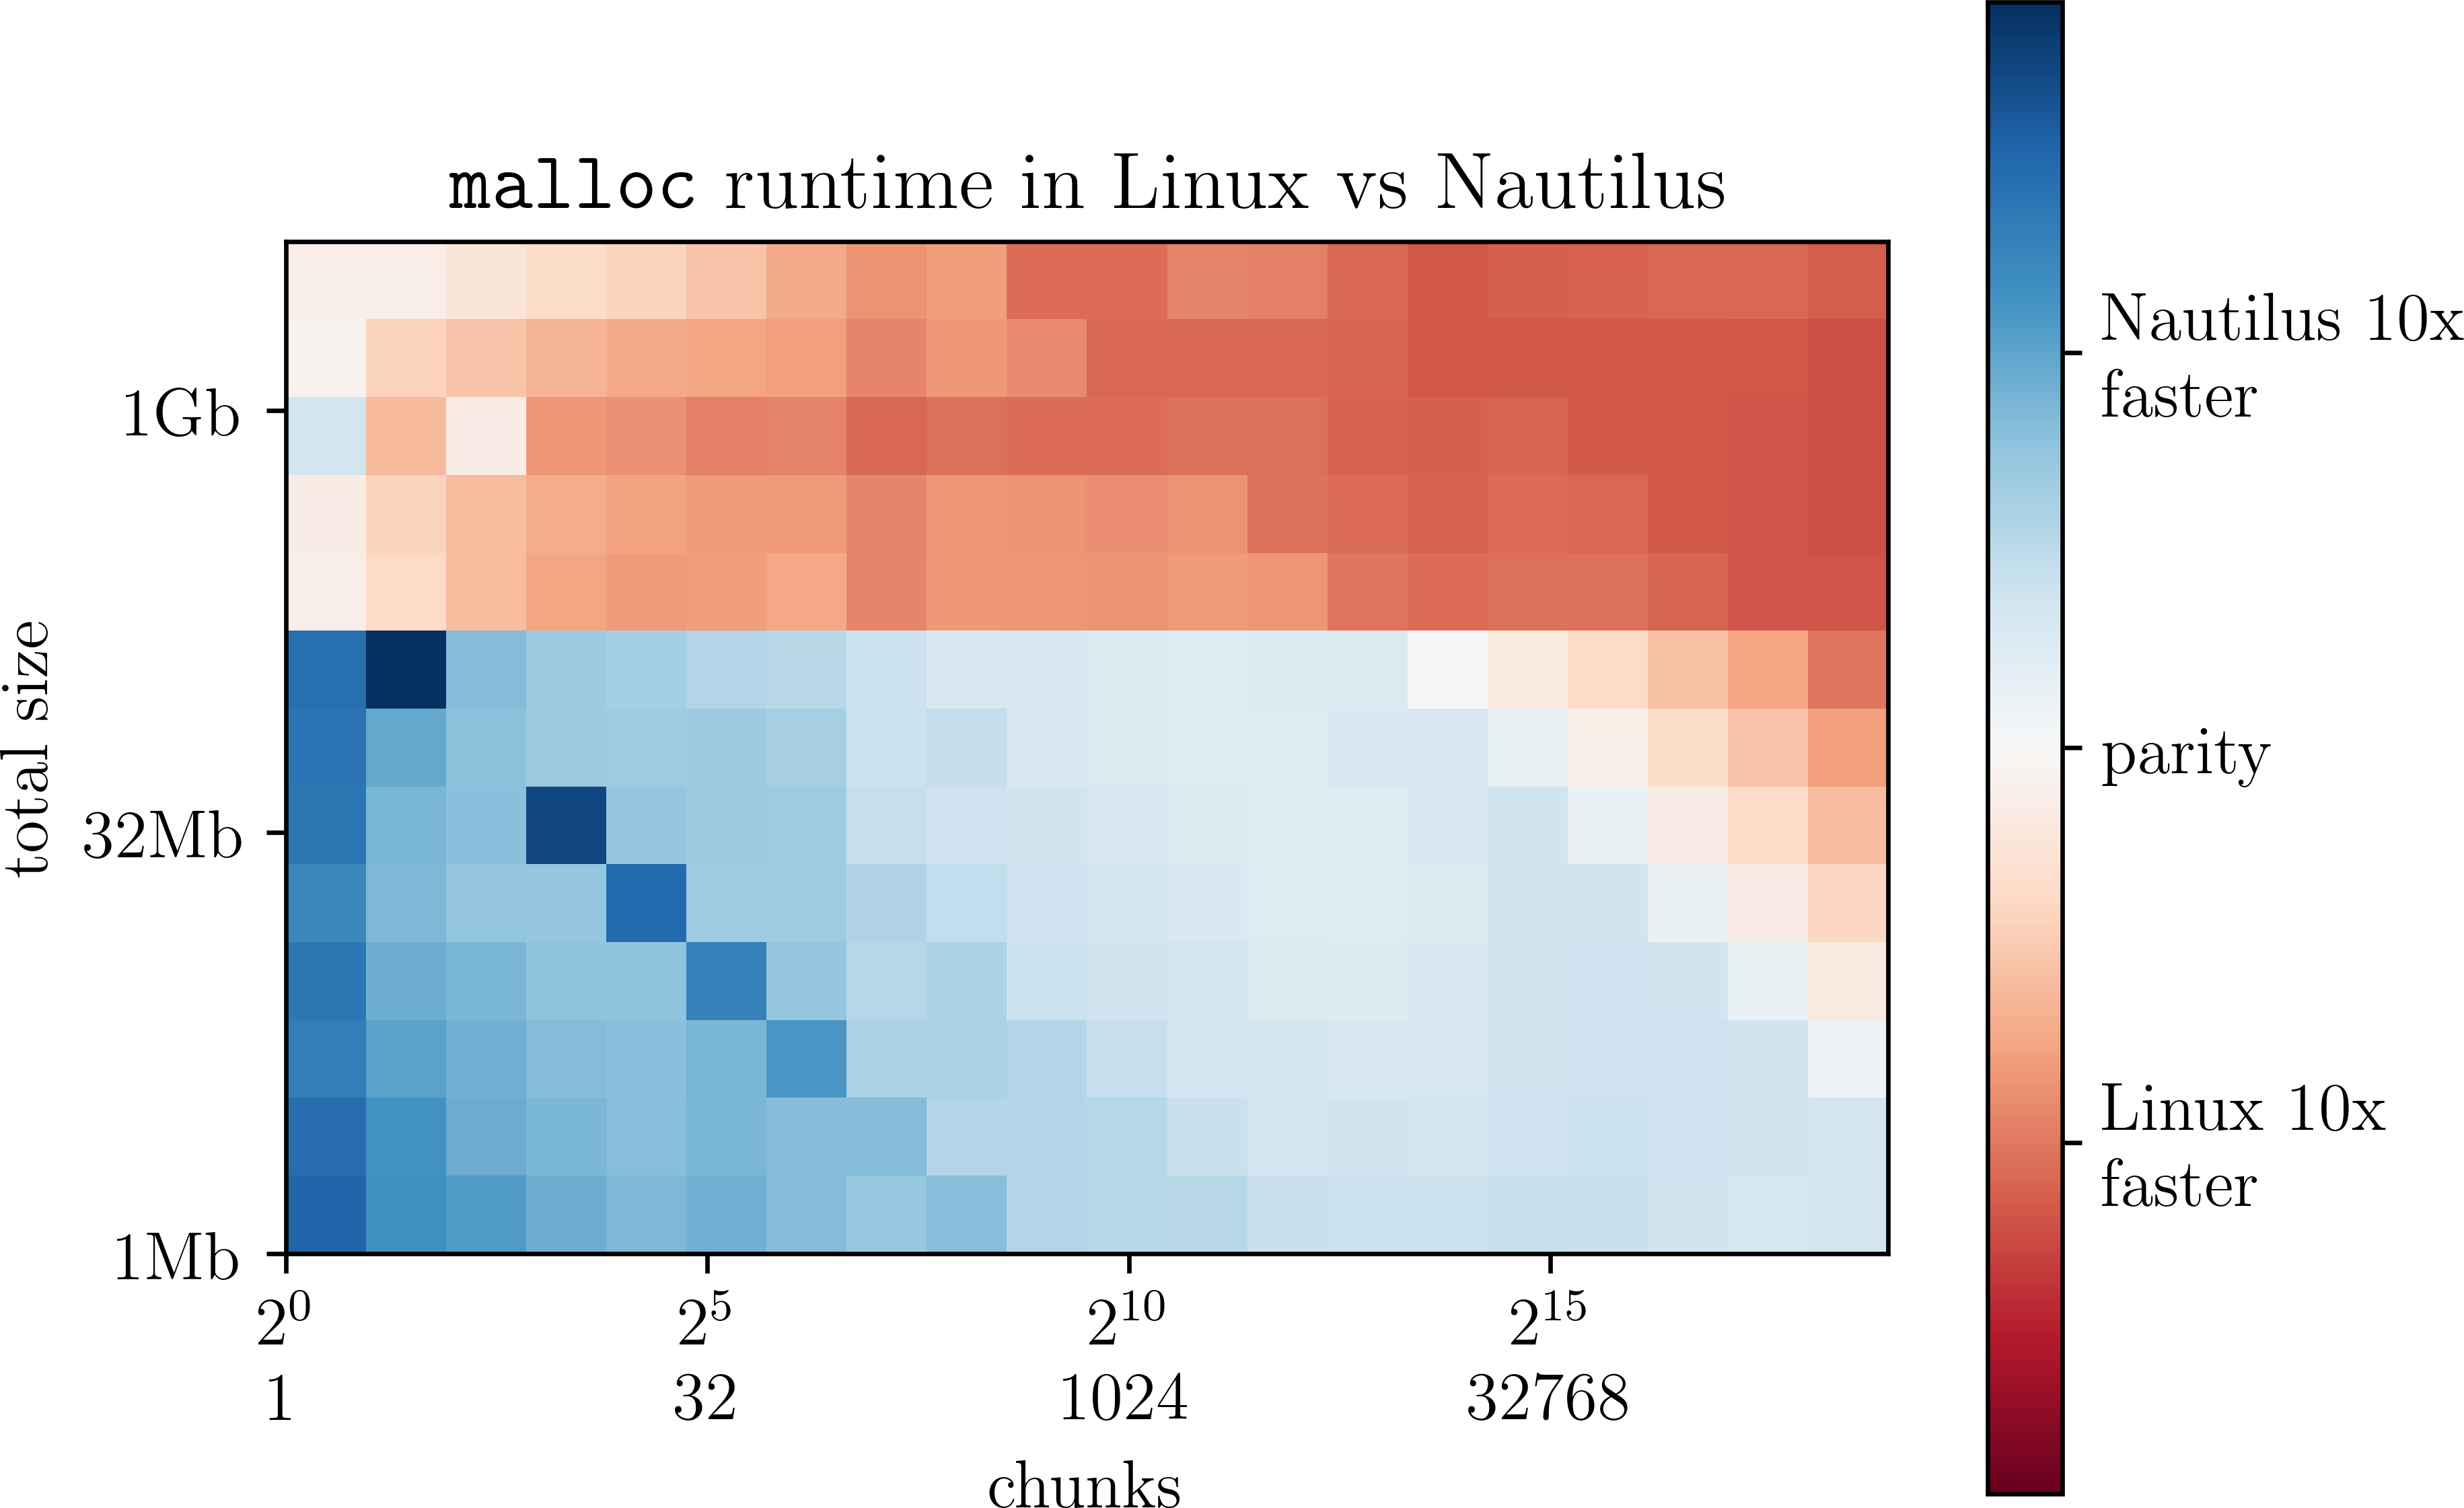
\includegraphics[height=30cm]{plots/malloc.png}
        \label{fig:1}
        \caption{Performance of allocating memory in chunks comparing linux against a custom memory allocator in Nautilus. Using specialization the custom allocator outperforms the highly optimized memory allocator of linux for smaller sizes by more than an order of magnitude. This demonstrates the potential of specialization - the behaviour of a component can be fine-tuned to workload characteristics.}
      \end{figure}
      \begin{block}{Our Vision: \textbf{NautDB}}
  
\end{block}

%%% Local Variables:
%%% mode: latex
%%% TeX-master: "main"
%%% End:

      \begin{block}{Previous Work}
  \begin{itemize}
      \item Customized OS support for data-processing~\cite{GICEVA:2016:OS_SUPPORT}: \todo{I am not sure what specific improvements we have over this paper.}
      \item A Case for Transforming Parallel Runtimes Into Operating System Kernels~\cite{HALE:2015:NAUTILUS}: the authors use a specialized runtime and show performance benefit for runtimes such as Legion.
      \item System-Level Support for Composition of Applications~\cite{KOCOLOSKI:2015:PISCES}: the authors introduce Pisces which allows multiple kernels to run on the same physical node, partitioning the resources. This makes it more convenient to run an single-application OS alongside a general-purpose OS for other applicatoins.
  \item Query compilation~\cite{SK16,N11} allows database engine code to be fine-tuned for individual queries
  \end{itemize}
  
\end{block}
%%% Local Variables:
%%% mode: latex
%%% TeX-master: "main"
%%% End:

      \begin{block}{NautDB Prototype}
  \begin{itemize}

  \item Hand-optimized, in-memory, columnar, chunk-oriented operator
    implementations

  \item Tables are stored in a column-oriented fashion, the data of a
    columns is split into 256 chunks - each is an array of data values
    of a fixed size

  \item We tested creating, sorting, selection (filter), creating, and
    freeing tables

  \item The database server is compiled into Nautilus and invoked on
    startup (single-application OS)

    % I don't want to get into these details.
    % They are important for the paper, but not for the poster
    % The reviewers said we needed more detail on other things, so I
    % will trade the space.
    % \item We report \textbf{sorting} a relation consisting of 256 chunks:
    %   \begin{itemize}
    %   \item intra chunk: sort data using counting sort
    %   \item inter chunk: merge sort
    %   \item two sorting variants: row-oriented versus column-oriented
    %   \end{itemize}
    %   splitting the input into chunks, applying counting sort per chunk, and merge sort to sort across chunks
    % \item Basic array operations: allocate, set all, get all, copy, and free

    %   \begin{itemize}

    %     these parameters are detailed is duplicated in the graph.
    %     No need for them here.
    %   \item \textbf{\# of columns}: between 2 and 128
    %   \item \textbf{\# of chunks}: 256
    %   \item \textbf{chunk size (\# of rows per chunk)}: between 256 ($2^8$) and 16,384 ($2^{14}$)
    %   \end{itemize}

  \end{itemize}
\end{block}

\begin{block}{Configuration}
  \begin{itemize}
  \item We vary the \underline{number of columns} and the \underline{size of chunks}
  \item We aggregated over 10 trials
  \item Hardware: 16-core x86\_64 AMD EPYC 7281 with 4 NUMA nodes
  \item OS: linux kernel 4.17.6, Nautilus - git commit \texttt{2fb4e52816}
  \item Nautilus has default configuration with debugging removed and extra devices disabled. It uses 1GB pages.
  \end{itemize}
\end{block}

%%% Local Variables:
%%% mode: latex
%%% TeX-master: "main"
%%% End:

    \end{column}

    % spacer column
    \begin{column}{\sepwid}
    \end{column}

    % column 3
    \begin{column}{\onecolwid}
      \begin{block}{Preliminary results I}
  Basic array operations (within a chunk) perform better in the specialized runtime.

  \begin{figure}
    
\includegraphics[height=20cm]{place_holder.png}
    \caption{Nautilus can reverse an array faster.}
  \end{figure}

  \begin{table}
    \begin{tabular}{l || c c | c c}
      Operation & Linux & & Nautilus & \\
      \hline\hline
      Allocate & 1.0e9 & 1.0x & 1.0e9 & 1.0x \\\hline
      Free & 1.0e9 & 1.0x & 1.0e9 & 1.0x \\\hline
      Copy (\texttt{memcpy}) & 1.0e9 & 1.0x & 1.0e9 & 1.0x \\\hline
      Copy (individually) & 1.0e9 & 1.0x & 1.0e9 & 1.0x \\\hline
      Reverse & 1.0e9 & 1.0x & 1.0e9 & 1.0x \\
    \end{tabular}

    Runtime measured in cycles according to \texttt{rdtsc}.

    \caption{Performance of Linux vs Nautilus on basic array operations averaged over 10 runs.}
  \end{table}
  
\end{block}
%%% Local Variables:
%%% mode: latex
%%% TeX-master: "main"
%%% End:

      \begin{block}{Preliminary results II - query processing primitives}

  Some operator implementations perform worse in the specialized runtime. We are researching why this is, and if there is a way to beat Linux's performance.
  
  \todo{Sort vary chunk size and num columns, parameters favorable to Nautilus}

  \todo{Select vary chunk size and num columns and domain size, parameters favorable to Nautilus}

  \todo{Create vary chunk size and num columns, parameters favorable to Nautilus}

\end{block}
%%% Local Variables:
%%% mode: latex
%%% TeX-master: "main"
%%% End:

    \end{column}

    % spacer column
    \begin{column}{\sepwid}
    \end{column}

    % column 4
    \begin{column}{\onecolwid}
      \begin{block}{Discussion}

  \begin{itemize}
  \item Preliminary experiments demonstrate that:
    \begin{itemize}
    \item Specialization allows operations to be tuned for a workload/application
    \item Compiled queries that consist of highly-specialized code benefit from a hybrid runtime environment
    \end{itemize}
  \item While Linux often outperforms our hybrid runtime, we can remedy this situation by introducing complementary specializations (as demonstrated in Fig.~\ref{fig:1})
  \end{itemize}

  \todo{
    Since we are specialized we can improve the performance for specific workloads.
    If we are not better, we could switch to different customizations (chosen by the application-programmer).
  }

\end{block}
%%% Local Variables:
%%% mode: latex
%%% TeX-master: "main"
%%% End:

      \begin{block}{Future Work}
  \begin{itemize}
  \item Implement performance counters (hardware-specific).
  \item Test more operators.
  \end{itemize}
\end{block}

%%% Local Variables:
%%% mode: latex
%%% TeX-master: "main"
%%% End:

      \begin{block}{Conclusion}
  The research is promising, but more work needs to be done. Future work should seek to understand and improve the preformance details such as TLB misses and data cache misses in order to beat a general purpose OS.

Making the process simpler from the application-programmer's perspective is an active topic of research.

\end{block}
%%% Local Variables:
%%% mode: latex
%%% TeX-master: "main"
%%% End:

      \begin{block}{References}
{\scriptsize
  \bibliographystyle{abbrv}
  \bibliography{kyle,sam,boris}
}

\end{block}

%%% Local Variables:
%%% mode: latex
%%% TeX-master: "main"
%%% End:

    \end{column}
    
  \end{columns}
  
\end{frame}

\end{document}

%%% Local Variables:
%%% mode: latex
%%% TeX-master: t
%%% End:
